%\documentclass[11pt,aspectratio=169]{beamer}
\documentclass[11pt,aspectratio=169,handout]{beamer}

\usepackage{amsmath}
\usepackage{amsfonts}
\usepackage{amssymb}
\usepackage{graphbox}
\usepackage{sgamevar}
\usepackage{pgfplots}
\usepackage{tikz}
\usepackage{pstricks,pst-node}
\usepackage{bigdelim}
\usepackage{qrcode}
\usepackage[absolute,overlay]{textpos}
\usepackage[ruled,vlined]{algorithm2e}



% alg
\SetKwFor{Repeat}{repeat}{}{}
\SetKwComment{Comment}{$\triangleright$ }{}
\SetCommentSty{textsf}
% pgfplot settings
\usepgfplotslibrary{fillbetween}

% tikz settings
\tikzset{
    invisible/.style={text opacity=1,opacity=0},
    visible on/.style={alt=#1{}{invisible}},
    alt/.code args={<#1>#2#3}{%
      \alt<#1>{\pgfkeysalso{#2}}{\pgfkeysalso{#3}}
    },
  }
\newcommand{\nebox}[2][]{\tikz[baseline=(h.base)]\node[rounded corners,rectangle,draw,line width=0.7pt,text depth=-4.9pt,#1] (h) {#2};}
\usetikzlibrary{arrows}
% Customized colors

\definecolor{ashgrey}{rgb}{0.7, 0.75, 0.71}
\definecolor{lightblue}{RGB}{140, 201, 247}
\definecolor{darkgreen}{RGB}{113, 160, 55}
\definecolor{darkblue}{RGB}{78, 103, 200}
\definecolor{darkpurple}{RGB}{112, 48, 160}

% Hyperlink settings

\hypersetup{colorlinks,urlcolor=darkgreen}

%Beamer settings

\setbeamertemplate{navigation symbols}{} 
\setbeamertemplate{footline}[frame number]
\setbeamertemplate{itemize items}[circle]
\setbeamertemplate{section in toc}[sections numbered]
\setbeamertemplate{subsection in toc}[subsection numbered]

\setbeamercolor{section in toc}{fg=blue}

\AtBeginSection[ ]{
 \begin{frame}{Outline}
  \hypersetup{linkcolor=black}
  \tableofcontents[currentsection]
 \end{frame}
}

% Graphics settings

\graphicspath{{../Figures/}}

% PGFPlot settings

\pgfplotsset{compat = newest}

% Gamesvar settings

\setlength{\arrayrulewidth}{0.91pt}
\renewcommand{\gamestretch}{1.68}
\def\stackedpayoffs#1#2{%
 \begin{array}{c}#1\\[2mm]#2\end{array}
}

% Math

\DeclareMathOperator*{\argmax}{argmax}
\DeclareMathOperator*{\argmin}{argmin}

\newcommand\given[1][]{\:#1\vert\:}
\newtheorem{proposition}{Proposition}

% New environments

\newenvironment{itemizes}[1][1em]{
 \vspace{#1}
 \begin{itemize}
 \setlength{\itemsep}{#1}
}{
 \end{itemize}
}


% Shared title frame

\title{Game-theoretic \\ Foundations of Multi-agent Systems}

\author{Seyed Majid Zahedi}
\titlegraphic{\vspace{-4.2em} 
\includegraphics[height=5.8em]{Logos/logo2}}

\date{} 
\subject{Lecture 1} 
\logo{
\includegraphics[height=5.6em]{Logos/logo1}}

\subtitle{\vspace{2.1em}Lecture 4: Computing Solution Concepts of Normal-form Games}

\begin{document}

 \begin{frame}[plain]
  \titlepage
 \end{frame}

 \section{Brief Overview of (Mixed Integer) Linear Programming}
  \begin{frame}{Example: Reproduction of Two Paintings}
   \begin{columns}
    \begin{column}{0.6\textwidth}
     \begin{center}
      \includegraphics<2->[width=0.2\textwidth]{L4/Picture1.jpg}
      \includegraphics<3->[width=0.2\textwidth]{L4/Picture2.jpg}
     \end{center}
     \begin{itemize}
      \item<2-> Painting 1 sells for \$30
      \item<3-> Painting 2 sells for \$20
      \item<4-> We have 16 units of {\color{blue} blue}, 8 {\color{darkgreen} green}, 5 {\color{red} red}
      \item<5-> Painting 1 requires 4 {\color{blue} blue}, 1 {\color{darkgreen} green}, 1 {\color{red} red}
      \item<6-> Painting 2 requires 2 {\color{blue} blue}, 2 {\color{darkgreen} green}, 1 {\color{red} red}
     \end{itemize}
    \end{column}
    \begin{column}<7->{0.25\textwidth}
     $$
      \begin{aligned}
       & \text{max.}
       & & 3x + 2y \\
       & \text{s.t.} & &  {\color{blue} 4x +2y \leq 16} \\
       & & &  {\color{darkgreen}x + 2y \leq 8} \\
       & & &  {\color{red} x + y \leq 5} \\
       & & &  x \ge 0 \\
       & & &  y \ge 0 \\
      \end{aligned}
     $$
    \end{column}
   \end{columns}
  \end{frame}
 
  \begin{frame}{Solving Linear Program Graphically}
   \begin{columns}
    \begin{column}<1->{0.25\textwidth}
     $$
      \begin{aligned}
       & \text{max.}
       & & 3x + 2y \\
       & \text{s.t.} & &  {\color{blue} 4x +2y \leq 16} \\
       & & &  {\color{darkgreen}x + 2y \leq 8} \\
       & & &  {\color{red} x + y \leq 5} \\
       & & &  x \ge 0 \\
       & & &  y \ge 0 \\
      \end{aligned}
     $$ 
    \end{column}
    \begin{column}<2->{0.7\textwidth}
     \begin{center}
      \begin{tikzpicture}
       \begin{axis}[
        width=0.7\textwidth, height=0.7\textwidth,
        axis line style={very thick, line cap=rect,},
        axis x line=bottom, axis y line=left,
        xmin=0, xmax=9, ymin=0, ymax=9,
        xtick=\empty, ytick=\empty,
        extra x ticks={2,4,6,8},
        extra x tick labels={2,4,6,8},
        extra x tick style ={font=\scriptsize},
        extra y ticks={2,4,6,8},
        extra y tick labels={2,4,6,8},
        extra y tick style ={font=\scriptsize},
        clip=false
       ]
        % add origin
        \coordinate (0) at (axis cs:0,0);
        \node [anchor=north east] at (0) {\scriptsize 0};
        
        \only<3->{\addplot [name path=b, darkblue, very thick, line cap=round, smooth, domain=0:4,]{-2*x + 8};}
        \only<4->{\addplot [darkgreen, very thick, line cap=round, smooth, domain=0:8, name path=g,]{-0.5*x + 4};}
        \only<5->{\addplot [red, very thick, line cap=round, smooth, domain=0:5, name path=r,]{-1*x + 5};}
        
        \only<6->{
         \path[name path=xaxis] (axis cs:0,0) -- (axis cs:4,0);
         \addplot[gray!80, opacity=0.4] fill between[of=g and xaxis , soft clip={domain=0:2}];
         \addplot[gray!80, opacity=0.4] fill between[of=r and xaxis , soft clip={domain=2:3}];
         \addplot[gray!80, opacity=0.4] fill between[of=b and xaxis , soft clip={domain=3:4}];
        }
        
        \only<7>{\addplot [gray, very thick, line cap=round, smooth,domain=0:2,]{-1.5*x+3};}
        
        \only<8->{\addplot [gray, very thick, line cap=round, smooth,domain=0:13/3,]{-1.5*x + 13/2};}
        \only<9->{
         \node[] at (axis cs: 6,4.5) {\shortstack{\scriptsize Optimal solution: $x=3$, $y=2$\\ \scriptsize  (objective 13)}};
         \draw [-latex, thick](axis cs: 5.5,4) -- (axis cs: 3.1,2.1);
        }
       \end{axis}
      \end{tikzpicture}
     \end{center}
    \end{column}
   \end{columns}
  \end{frame}
 
  \begin{frame}{Modified LP}
   \begin{columns}
    \begin{column}{0.25\textwidth}
     $$
      \begin{aligned}
       & \text{max.}
       & & 3x + 2y \\
       \only<1>{& \text{s.t.} & &  {\color{blue} 4x +2y \leq 16} \\}
       \only<2->{& \text{s.t.} & &  {\color{blue} 4x +2y \leq 15} \\}
       & & &  {\color{darkgreen}x + 2y \leq 8} \\
       & & &  {\color{red} x + y \leq 5} \\
       & & &  x \ge 0 \\
       & & &  y \ge 0 \\
      \end{aligned}
     $$
     \begin{tikzpicture}[overlay]
      \only<3->{\draw [darkpurple, dashed, ultra thick] (3.2,3) circle (9pt);}
     \end{tikzpicture}
    \end{column}
    \begin{column}{0.5\textwidth}
     \begin{itemizes}
      \item<4-> Optimal solution: x = 2.5, y = 2.5
      \item<5-> Objective = 7.5 + 5 = 12.5
      \item<6-> Can we sell half paintings?
     \end{itemizes}
    \end{column}
   \end{columns}
  \end{frame}
 
  \begin{frame}{Integer Linear Program}
   \begin{columns}<1->
    \begin{column}{0.25\textwidth}
     $$
      \begin{aligned}
       & \text{max.}
       & & 3x + 2y \\
       & \text{s.t.} & &  {\color{blue} 4x +2y \leq 15} \\
       & & &  {\color{darkgreen}x + 2y \leq 8} \\
       & & &  {\color{red} x + y \leq 5} \\
       & & &  x \in \mathbb{N}_{0}\\
       & & &  y \in \mathbb{N}_{0} \\
      \end{aligned}
     $$
    \end{column}
    \begin{column}{0.7\textwidth}
     \begin{center}
      \begin{tikzpicture}
       \begin{axis}[
        width=0.7\textwidth, height=0.7\textwidth,
        axis line style={very thick, line cap=rect,},
        axis x line=bottom, axis y line=left,
        xmin=0, xmax=9, ymin=0, ymax=9,
        xtick=\empty, ytick=\empty,
        extra x ticks={2,4,6,8},
        extra x tick labels={2,4,6,8},
        extra x tick style ={font=\scriptsize},
        extra y ticks={2,4,6,8},
        extra y tick labels={2,4,6,8},
        extra y tick style ={font=\scriptsize},
        clip=false
       ]
        \addplot [darkblue, very thick, line cap=round, smooth,domain=0:3.75,] {-2*x + 7.5};
        \addplot [darkgreen, very thick, line cap=round, smooth, domain=0:8,]{-0.5*x + 4};
        \addplot [red, very thick, line cap=round, smooth, domain=0:5,]{-1*x + 5};
        \only<2->{\addplot [gray, very thick, line cap=round, dashed,domain=0:12.5/3,]{-1.5*x + 6.25};}
        \coordinate (0) at (axis cs:0,0);
        \coordinate (1) at (axis cs:0,1);
        \coordinate (2) at (axis cs:1,0);
        \coordinate (3) at (axis cs:1,1);
        \coordinate (4) at (axis cs:0,2);
        \coordinate (5) at (axis cs:2,0);
        \coordinate (6) at (axis cs:2,1);
        \coordinate (7) at (axis cs:1,2);
        \coordinate (8) at (axis cs:2,2);
        \coordinate (9) at (axis cs:0,3);
        \coordinate (10) at (axis cs:3,0);
        \coordinate (11) at (axis cs:0,4);
        \coordinate (12) at (axis cs:1,3);
        \coordinate (13) at (axis cs:2,3);
        \coordinate (14) at (axis cs:3,1);
        % add origin
        \node [anchor=north east] at (0) {\scriptsize 0};
        
        \only<3->{
         \node[] at (axis cs: 5.3,5.2) {\shortstack{\scriptsize Optimal LP solution:\\ \scriptsize $x = 2.5$, $y = 2.5$ \\ \scriptsize (objective 12.5)}};
         \draw [-latex, thick](axis cs: 4.9,4.3) -- (axis cs: 2.6,2.6);
        }
        
        \only<5->{
         \node[] at (axis cs: 2.5,7) {\shortstack{\scriptsize Optimal ILP solution:\\ \scriptsize $x = 2$, $y = 3$ \\ \scriptsize (objective 12)}};
         \draw [-latex, thick](axis cs: 2.2,6) -- (axis cs: 2,3.25);
        }
       \end{axis}
       \only<4->{
         \foreach \n in {0,1,2,3,4,5,6,7,8,9,10,11,12,13,14}
         \filldraw[color=black, fill=lightblue, very thick](\n) circle (2.5pt);
       }
      \end{tikzpicture}
     \end{center}
    \end{column}
   \end{columns}
  \end{frame}
 
  \begin{frame}{Mixed Integer Linear Program}
   \begin{columns}<1->
    \begin{column}{0.25\textwidth}
     $$
      \begin{aligned}
       & \text{max.}
       & & 3x + 2y \\
       & \text{s.t.} & &  {\color{blue} 4x +2y \leq 15} \\
       & & &  {\color{darkgreen}x + 2y \leq 8} \\
       & & &  {\color{red} x + y \leq 5} \\
       & & &  x \ge 0 \\
       & & &  y \in \mathbb{N}_{0} \\
      \end{aligned}
     $$
    \end{column}
    \begin{column}{0.7\textwidth}
     \begin{center}
      \begin{tikzpicture}
       \begin{axis}[
        width=0.7\textwidth, height=0.7\textwidth,
        axis line style={very thick, line cap=rect,},
        axis x line=bottom, axis y line=left,
        xmin=0, xmax=9, ymin=0, ymax=9,
        xtick=\empty, ytick=\empty,
        extra x ticks={2,4,6,8},
        extra x tick labels={2,4,6,8},
        extra x tick style ={font=\scriptsize},
        extra y ticks={2,4,6,8},
        extra y tick labels={2,4,6,8},
        extra y tick style ={font=\scriptsize},
        clip=false
       ]
        \addplot [darkblue, very thick, line cap=round, smooth,domain=0:3.75,]{-2*x + 7.5};
        \addplot [darkgreen, very thick, line cap=round, smooth, domain=0:8,]{-0.5*x + 4};
        \addplot [red, very thick, line cap=round, smooth, domain=0:5,]{-1*x + 5};
        \addplot [gray, very thick, line cap=round, dashed,domain=0:12.5/3,] {-1.5*x + 6.25};
    
        \coordinate (0) at (axis cs:0,0);
        \coordinate (1) at (axis cs:0,1);
        \coordinate (2) at (axis cs:0,2);
        \coordinate (3) at (axis cs:0,3);
        \coordinate (4) at (axis cs:0,4);
        \coordinate (5) at (axis cs:2,3);
        \coordinate (6) at (axis cs:15/4,0);
        \coordinate (7) at (axis cs:13/4,1);
        \coordinate (8) at (axis cs:11/4,2);
    
        \node[] at (axis cs: 2.5,7) {\shortstack{\scriptsize Optimal ILP solution:\\ \scriptsize $x = 2$, $y = 3$ \\ \scriptsize (objective 12)}};
        \draw [-latex, thick](axis cs: 2.2,6) -- (axis cs: 2,3.25);
        \node[] at (axis cs: 5.3,5.2) {\shortstack{\scriptsize Optimal LP solution:\\ \scriptsize $x = 2.5$, $y = 2.5$ \\ \scriptsize (objective 12.5)}};
        \draw [-latex, thick](axis cs: 4.9,4.3) -- (axis cs: 2.6,2.6);
        
        \only<3->{
         \node[] at (axis cs: 8,3.2) {\shortstack{\scriptsize Optimal MILP \\\scriptsize solution: $x = 2.75$, $y = 2$ \\ \scriptsize (objective 12.25)}};
         \draw [-latex, thick](axis cs: 5.8,2.7) -- (axis cs: 2.9,2);
        }
        % add origin
        \node [anchor=north east] at (0) {\scriptsize 0};
       \end{axis}
       \only<2->{
        \draw[lightblue, line width=2pt] (0) -- (6);
        \draw[lightblue, line width=2pt] (1) -- (7);
        \draw[lightblue, line width=2pt] (2) -- (8);
        \draw[lightblue, line width=2pt] (3) -- (5);
        \foreach \n in {0,1,2,3,4,5,6,7,8}
         \filldraw[color=black, fill=lightblue, very thick](\n) circle (2.5pt);
       }
      \end{tikzpicture}
     \end{center}
    \end{column}
   \end{columns}
  \end{frame}
 
  \begin{frame}{Solving Mixed Linear/Integer Programs}
   \begin{itemize}[<+->]
   \setlength{\itemsep}{1.5em}
    \item Linear programs can be solved efficiently
    \begin{itemize}
     \item Simplex, ellipsoid, interior point methods, etc.
    \end{itemize}
    \item (Mixed) integer programs are \alert{NP-hard} to solve
    \begin{itemize}
     \item Many standard NP-complete problems can be modeled as MILP
     \item Search type algorithms such as branch and bound
    \end{itemize}
    \item Standard packages for solving these
    \begin{itemize}
     \item Gurobi, MOSEK, GNU Linear Programming Kit, CPLEX, CVXOPT, etc.
    \end{itemize}
    \item LP relaxation of (M)ILP: remove integrality constraints
    \begin{itemize}
     \item Gives upper bound on MILP ($\sim$ admissible heuristic)
    \end{itemize}
   \end{itemize}
  \end{frame}
 
  \begin{frame}{Exercise I: Knapsack-type Problem}
   \begin{itemize}
    \item We arrive in room full of precious objects
    \item Can carry only 30kg out of the room
    \item Can carry only 20 liters out of the room
    \item Want to maximize our total value
    \item Unit of object A: 16kg, 3 liters, sells for \$11 (3 units available)
    \item Unit of object B: 4kg, 4 liters, sells for \$4 (4 units available)
    \item Unit of object C: 6kg, 3 liters, sells for \$9 (1 unit available)
    \item What should we take?
   \end{itemize}
  \end{frame}
 
  \begin{frame}{Exercise II: Cellphones (Set Cover)}
   \begin{itemize}
    \item We want to have a working phone in every continent (besides Antarctica) 
    \item But we want to have as few phones as possible
    \item Phone A works in NA, SA, Af
    \item Phone B works in E, Af, As
    \item Phone C works in NA, Au, E
    \item Phone D works in SA, As, E
    \item Phone E works in Af, As, Au
    \item Phone F works in NA, E
   \end{itemize}
  \end{frame}
 
  \begin{frame}{Exercise III: Hot-dog Stands}
   \begin{itemize}
    \item We have two hot-dog stands to be placed in somewhere along beach
    \item We know where groups of people who like hot dogs are
    \item We also know how far each group is willing to walk
    \item Where do we put our stands to maximize \# hot dogs sold? (price is fixed)
   \end{itemize}
   \vspace{3.5em}
   \begin{columns}
    \begin{column}{0.9\textwidth}
     \begin{tikzpicture}
      \only<2->{
       \draw[black, ultra thick] (0,0) -- (12,0);
       \draw [black,fill=darkblue, ultra thick] (0.75,0) circle (2.5pt);
       \node[anchor=north] at (3/4,-0.2) {\shortstack{\tiny \underline{Group 1} \\ \tiny location: 1 \\ \tiny size: 2 \\ \tiny walk dist.: 4}};
      }
      \only<3->{
       \draw [black,fill=darkblue, ultra thick] (3,0) circle (2.5pt);
       \node[anchor=north] at (12/4,-0.2) {\shortstack{\tiny \underline{Group 2} \\ \tiny location: 4 \\ \tiny size: 1 \\ \tiny walk dist.: 2}};
       \draw [black,fill=darkblue, ultra thick] (21/4,0) circle (2.5pt);
       \node[anchor=north] at (21/4,-0.2) {\shortstack{\tiny \underline{Group 3} \\ \tiny location: 7 \\ \tiny size: 3 \\ \tiny walk dist: 3}};
       \draw [black,fill=darkblue, ultra thick] (27/4,0) circle (2.5pt);
       \node[anchor=north] at (27/4,-0.2) {\shortstack{\tiny \underline{Group 4} \\ \tiny location: 9 \\ \tiny size: 4 \\ \tiny walk dist.: 3}};
       \draw [black,fill=darkblue, ultra thick] (45/4,0) circle (2.5pt);
       \node[anchor=north] at (45/4,-0.2) {\shortstack{\tiny \underline{Group 5} \\ \tiny location: 15 \\ \tiny size: 3 \\ \tiny walk dist.: 2}};
      }
     \end{tikzpicture}
    \end{column}
   \end{columns}
  \end{frame}
 
 \section{Dominated Strategies}
  \begin{frame}{Dominance by Pure Strategy}
   \begin{algorithm*}[H]
    \For{all $a_i \in A_i$ where $a_i \ne s_i$}{
     \textit{dom} $\leftarrow$ \textit{true}\;
     \ForAll{$a_{-i} \in A_{-i}$}{
      \If{$u_i(s_i, a_{-i}) \ge u_i(a_i, a_{-i})$}{
       \textit{dom} $\leftarrow$ \textit{false}\;
       \textbf{break}\;
      }
     }
     \If{\textit{dom} $=$ \textit{true}}{
      \Return \textit{true}\;
     }
    }
    \Return \textit{false}\;
   \label{alg:IDS}
   \caption{Determine whether $s_i$ is strictly dominated by any pure strategy}
   \end{algorithm*}
  \end{frame}
  
  \begin{frame}{Recall: Strict Dominance}
   \begin{center}
    $a_i$ \alert{strictly dominates} $s_i$ if $u_i(a_i, s_{-i}) > u_i(s_i,s_{-i})$ $\forall s_{-i} \in S_{-i}$
   \end{center}
  \end{frame}
    
  \begin{frame}{Dominance by Pure Strategy: Discussion}
   \begin{itemize}[<+->]
   \setlength{\itemsep}{1.2em}
    \item Complexity of the Algorithm is $O(\vert A\vert)$, linear in the size of normal-form game
    \item Recall: $a_i$ \alert{strictly dominates} $s_i$ if $u_i(a_i, s_{-i}) > u_i(s_i,s_{-i})$ $\forall s_{-i} \in S_{-i}$
    \item<.-> This definition refers to mixed-strategy profile of other agents
    \item In Alg. (\ref{alg:IDS}), we do not check every mixed-strategy profile of others, why?
    \begin{itemize}
    \setlength{\itemsep}{0.8em}
     \item Suppose $a_i$ does not strictly dominate $s_i$ for all $a_{-i}$
     \item Then, there is no $s_{-i}$ for which $a_i$ strictly dominates $s_i$
     \item This holds because of the linearity of expectation
    \end{itemize}
   \end{itemize}
  \end{frame}
  
  \begin{frame}{Weak Dominance by Mixed Strategy}
   \begin{itemize}
    \item<1-> Checking if strategy $s_i$ is weakly dominated by any mixed strategy
    \begin{equation*}
     \begin{aligned}
      \visible<3->{& \text{max.} & & \sum_{a_{-i}\in A_{-i}}\left[\left(\sum_{a_i \in A} p_{a_i} u_{i}(a_i, a_{-i})\right) - u_i(s_i, a_{-i})\right] &\\}
      \visible<2->{& \text{s.t.} & &  \sum_{a_i\in A_i} p_{a_i} u_i(a_i,a_{-i}) \ge u_i(s_i,a_{-i}) & \forall a_{-i}\in A_{-i} \\
      & & &  \sum_{a_i\in A_i}p_{a_i} = 1 & \\
      & & &  p_{a_i} \ge 0, & \forall a_i \in A_i \\}
     \end{aligned} 
    \end{equation*}
    \item<4> If optimal solution is strictly positive, then $s_i$ is weakly dominated by $\{p_{a_i}\}$
   \end{itemize}
  \end{frame}  
  
  \begin{frame}{Strict Dominance by Mixed Strategies}
   \begin{itemize}
    \item<1-> Checking if strategy $s_i$ is strictly dominated by any mixed strategy
    \begin{equation*}
     \begin{aligned}
      \visible<4->{& \text{max.} & & \epsilon &\\}
      \visible<2->{& \text{s.t.} & &  \sum_{a_i\in A_i} p_{a_i} u_i(a_i,a_{-i}) \ge u_i(s_i,a_{-i}) + \epsilon & \forall a_{-i}\in A_{-i} \\}
      \visible<3->{& & &  \sum_{a_i\in A_i}p_{a_i} = 1 & \\
      & & &  p_{a_i} \ge 0, & \forall a_i \in A_i \\}
     \end{aligned} 
    \end{equation*}
    \item<5-> If optimal solution is strictly positive, then $s_i$ is strictly dominated by $\{p_{a_i}\}$
   \end{itemize}
  \end{frame} 
  
  \begin{frame}{Path Dependency of Iterated Dominance}
   \begin{itemize}
    \item<1-> Iterated weak dominance is \alert{path-dependent}:
    \begin{itemize}
     \item<1-> Sequence of eliminations may determine which solution we get (if any)
    \end{itemize}
    \begin{columns}
    \hspace{5em}
     \begin{column}<2->{0.3\textwidth}
      \begin{tikzpicture}[overlay]
       \coordinate (A) at (0.74, -0.67);
       \coordinate (B) at (1.74, -0.67);
       \coordinate (C) at (0.24, -1.72);
       \coordinate (D) at (0.24, -1.82);
       \coordinate (E) at (0.24, -0.97);
       \coordinate (F) at (0.24, -2.57);
       \only<5->{\draw[-latex, red, line width=3pt] (B)to[out=100,in=80, looseness=2](A);}
       \only<3->{\draw[-latex, red, line width=3pt] (C)to[out=180,in=-180, looseness=2.5](E);}
       \only<7->{\draw[-latex, red, line width=3pt] (D)to[out=180,in=-180, looseness=2.5](F);}
     
       \coordinate (0) at (0.74+4.55, -0.67);
       \coordinate (1) at (1.74+4.55, -0.67);
       \coordinate (2) at (0.24+4.55, -1.72);
       \coordinate (3) at (0.24+4.55, -1.82);
       \coordinate (4) at (0.24+4.55, -0.97);
       \coordinate (5) at (0.24+4.55, -2.57);
       \only<12->{\draw[-latex, red, line width=3pt] (0)to[out=100,in=80, looseness=2](1);}
       \only<14->{\draw[-latex, red, line width=3pt] (2)to[out=180,in=-180, looseness=2.5](4);}
       \only<10->{\draw[-latex, red, line width=3pt] (3)to[out=180,in=-180, looseness=2.5](5);}
     
       \coordinate (a) at (0.24+4.55*2, -1.72);
       \coordinate (b) at (0.24+4.55*2, -1.82);
       \coordinate (c) at (0.24+4.55*2, -0.97);
       \coordinate (d) at (0.24+4.55*2, -2.57);
       \only<17->{\draw[-latex, red, line width=3pt] (a)to[out=180,in=-180, looseness=2.5](c);
       \draw[-latex, red, line width=3pt] (b)to[out=180,in=-180, looseness=2.5](d);}
       
       \only<4->{\draw[red, thick] (0.24,-0.67)--(2.22,-1.42);
       \draw[red, thick] (0.24,-1.42)--(2.22,-0.67);}
       \only<6->{\draw[red, thick] (0.24,-0.67)--(0.24+0.99,-0.67-3*0.75);
       \draw[red, thick] (0.24,-0.67-3*0.75)--(0.24+0.99,-0.67);}
       \only<8->{\draw[red, thick] (0.24,-0.67-1.5)--(2.22,-1.42-1.5);
       \draw[red, thick] (0.24,-1.42-1.5)--(2.22,-0.67-1.5);}
     
       \only<15->{\draw[red, thick] (0.24+4.55,-0.67)--(2.22+4.55,-1.42);
       \draw[red, thick] (0.24+4.55,-1.42)--(2.22+4.55,-0.67);}
       \only<13->{\draw[red, thick] (0.24+4.55+0.99,-0.67)--(0.24+0.99+4.55+0.99,-0.67-3*0.75);
       \draw[red, thick] (0.24+4.55+0.99,-0.67-3*0.75)--(0.24+0.99+4.55+0.99,-0.67);}
       \only<11->{\draw[red, thick] (0.24+4.55,-0.67-1.5)--(2.22+4.55,-1.42-1.5);
       \draw[red, thick] (0.24+4.55,-1.42-1.5)--(2.22+4.55,-0.67-1.5);}
     
       \only<18->{\draw[red, thick] (0.24+4.55*2,-0.67)--(2.22+4.55*2,-1.42);
       \draw[red, thick] (0.24+4.55*2,-1.42)--(2.22+4.55*2,-0.67);
       \draw[red, thick] (0.24+4.55*2,-0.67-1.5)--(2.22+4.55*2,-1.42-1.5);
       \draw[red, thick] (0.24+4.55*2,-1.42-1.5)--(2.22+4.55*2,-0.67-1.5);}
      \end{tikzpicture}
      
      \begin{game}{3}{2}
       \>     \>   \\
       \> $0,1$ \> $1,0$  \\
       \> $1,0$ \> $1,0$  \\
       \> $1,0$ \> $0,1$ 
      \end{game}
     \end{column}
     \begin{column}<9->{0.3\textwidth}
      \begin{game}{3}{2}
       \>     \>   \\
       \> $0,1$ \> $1,0$  \\
       \> $1,0$ \> $1,0$  \\
       \> $1,0$ \> $0,1$ 
      \end{game}
     \end{column}
     \begin{column}<16->{0.3\textwidth}
      \begin{game}{3}{2}
       \>     \>   \\
       \> $0,1$ \> $1,0$  \\
       \> $1,0$ \> $1,0$  \\
       \> $1,0$ \> $0,1$ 
      \end{game}
     \end{column}
     \end{columns}
     \vspace{2em}
     \item<19-> Iterated strict dominance is \alert{path-independent}:
     \begin{itemize}
      \item<19-> Elimination process will always terminate at the same point
     \end{itemize}
    \end{itemize}
   \end{frame}
 
   \begin{frame}{Computational Questions for Iterated Dominance}
    \begin{itemize}[<+->]
    \setlength{\itemsep}{1.2em}
     \item Is there some elimination path under which $s_i$ is eliminated?
     \item Is there maximally reduced game where each agent has exactly 1 action?
     \item For \alert{strict dominance}, both can be solved in polynomial time
     \begin{itemize}[<.->]
      \item Due to path-independence
      \item Check if any strategy is dominated, remove it, repeat
      \item With or without dominance by mixed strategies
     \end{itemize} 
     \item For \alert{weak dominance}, both questions are NP-hard%
      \footnote<4->{\scriptsize[Conitzer, Sandholm 05] and weaker version proved by [Gilboa, Kalai, Zemel 93]}
     \begin{itemize}[<.->]
      \item Even when all utilities are 0 or 1
      \item With or without dominance by mixed strategies
     \end{itemize}
    \end{itemize}
   \end{frame}
   
 \section{Minmax and Maxmin Strategies}
  \begin{frame}{Recall: Minmax and Maxmin}
   \begin{itemize}
    \item<1-> \alert{Maxmin} strategy for agent $i$ (maxmin value for agent $i$)
    $$
     \argmax_{s_i} \min_{s_{-i}} u_i(s_i, s_{-i})
    $$
    \item<2-> \alert{Minmax} strategy against agent $i$ (minmax value for agent $i$)
    $$
     \argmin_{s_{-i}} \max_{s_{i}} u_i(s_i, s_{-i})
    $$
   \end{itemize}
  \end{frame}
  

  \begin{frame}{Maxmin Strategy and Value}
   \begin{itemize}
    \item<1-> Finding maxmin strategy of agent $i$
    $$
     \begin{aligned}
      \visible<4->{& \text{max.} & & U_i & \\}
      \visible<2->{& \text{s.t.} & &  \sum_{a_i\in A_i}p_{a_i} u_i(a_i,a_{-i}) \ge U_i, & \forall a_{-i}\in A_{-i} \\}
      \visible<3->{& & &  \sum_{a_i\in A_i}p_{a_i} = 1 & \\
      & & &  p_{a_i} \ge 0,  & \forall a_i \in A_i \\}
     \end{aligned}
    $$
    \item<2-> Given $p_{a_i}$, first constraint ensures that $U_i$ is less than any achievable expected utility for any pure strategies of opponents
    \item<4-> Objective of this LP, $U_i$, is \alert{maxmin value} of agent $i$
   \end{itemize}
  \end{frame}

  
 \section{Nash Equilibrium}
  \begin{frame}{NE of Two-player, Zero-sum Games}
   \begin{columns}
   \hspace{0.5em}
    \begin{column}{0.49\textwidth}
     \begin{itemize}
      \item<1-> Maximin value for agent 1
      \vspace{0.5em}
      \onslide<2->{\footnotesize 
       $$
        \begin{aligned}
         & \text{max.}
         & & U_{1} & \\
         & \text{s.t.} & &  \sum_{a_1\in A_1}p_{a_1} u_1(a_1,a_2) \ge U_1 & \forall a_2\in A_2 \\
         & & &  \sum_{a_1\in A_1}p_{a_1} = 1 & \\
         & & &  p_{a_1} \ge 0,  & \forall a_1 \in A_1 \\
        \end{aligned}
       $$
      }
     \end{itemize}     
    \end{column}
    \begin{column}{0.49\textwidth}
     \begin{itemize}
      \item<3-> Minmax value for agent 1
      \vspace{0.5em}
      \onslide<4->{\footnotesize
       $$
        \begin{aligned}
         & \text{min.}
         & & U_{1} & \\
         & \text{s.t.} & &  \sum_{a_2\in A_2}p_{a_2} u_1(a_1,a_2) \le U_1 & \forall a_1\in A_1 \\
         & & &  \sum_{a_2\in A_2}p_{a_2} = 1 & \\
         & & &  p_{a_2} \ge 0,  & \forall a_2 \in A_2 \\
        \end{aligned}
       $$
      }       
     \end{itemize}
    \end{column}
   \end{columns}
   \begin{itemize}
    \item<5-> NE is expressed as \alert{LP} $\Rightarrow$ NE can be computed in \alert{polynomial time}
   \end{itemize}
  \end{frame}
  
  \begin{frame}{Maximin Strategy for General-sum Games}
   \begin{itemize}
    \item<1-> Agents could still play minimax strategy in general-sum games
    \begin{itemize}
     \item<2-> I.e., pretend that the opponent is only trying to hurt you
    \end{itemize}
    \item<3-> But this might not be rational:
    \onslide<4->
    \begin{center}
    \hspace{-5em}
     \begin{game}{2}{2}[Agent 1][Agent 2]
         \> Left   \> Right  \\
      Up \> $0,0$ \> $3,1$ \\
      Down \> $1,0$ \> $2,1$
     \end{game}
    \end{center}
    \vspace{1 em}
    \begin{itemize}
     \item<5-> If A2 was trying to hurt A1, she would play Left, so A1 should play Down
     \item<6-> In reality, A2 will play Right (strictly dominant), so A1 should play Up
    \end{itemize}
   \end{itemize}
  \end{frame}

  \begin{frame}{Hardness of Computing NE for General-sum Games }
   \begin{itemize}[<+->]
    \item Complexity was open for long time
    \begin{itemize}
     \item<.-> “together with factoring […] the most important concrete open question on
the boundary of P today” {\scriptsize \color[rgb]{0.29, 0.59, 0.9} [Papadimitriou STOC’01]}
    \end{itemize}
    \item Sequence of papers showed that computing any NE is PPAD-complete
(even in 2-player games) {\scriptsize \color[rgb]{0.29, 0.59, 0.9} [Daskalakis, Goldberg, Papadimitriou 2006; Chen, Deng 2006]}
    \item All known algorithms require \alert{exponential time} (in worst case)
   \end{itemize}
  \end{frame}

  \begin{frame}{Hardness of Computing NE for General-Sum Games (cont.)}
   \begin{itemize}[<+->]
    \item What about computing NE with \alert{specific property}?
    \begin{itemize}[<.->]
     \item NE that is not Pareto-dominated
     \item NE that maximizes expected social welfare (i.e., sum of all agents’ utilities)
     \item NE that maximizes expected utility of given agent
     \item NE that maximizes expected utility of worst-off player
     \item NE in which given pure strategy is played with positive probability
     \item NE in which given pure strategy is played with zero probability
     \item …
    \end{itemize}
    \item All of these are NP-hard (and the optimization questions are
 inapproximable assuming P != NP), even in 2-player games \\
 {\scriptsize [Gilboa, Zemel 89; Conitzer \& Sandholm IJCAI-03/GEB-08]}
   \end{itemize}
  \end{frame}

  \begin{frame}{Search-based Approaches (for Two-player Games)}
   \begin{itemize}
    \item<1-> We can use LP, if we know support $X_i$ of each player $i$’s mixed strategy
    \visible<2->{\scriptsize
     $$
      \begin{aligned}
       & \text{find}
       & & (U_1, U_2) & \\
       & \text{s.t.} & & p_{a_i} \ge 0, & \forall i, a_i \in A_i \\
       & & &\sum_{a_i \in A_i} p_{a_i} = 1, & \forall i \\
       & & & p_{a_i} = 0, & \forall i, a_i \in A_i/X_i \\
       & & & \sum_{a_{-i} \in A_{-i}}p_{a_{-i}}u_i(a_i,a_{-i}) = U_i, & \forall i, a_i \in X_i \\
       & & & \sum_{a_{-i} \in A_{-i}}p_{a_{-i}}u_i(a_i,a_{-i}) \le U_i, & \forall i, a_i \in A_i/X_i \\
      \end{aligned}
     $$
    }
    \item<3-> Thus, we can search over possible supports, which is basic idea underlying methods in {\scriptsize \color[rgb]{0.29, 0.59, 0.9} [Dickhaut \& Kaplan 91; Porter, Nudelman, Shoham AAAI04/GEB08]}
   \end{itemize}
  \end{frame}

  \begin{frame}{NE using MILP (for Two-player Games) \\{\small [Sandholm, Gilpin, Conitzer AAAI05]
}}
   \begin{columns}<1->
    \begin{column}{0.7\textwidth}
    {\small
     $$
      \begin{aligned}
       & \text{max.}
       & & \text{whatever you like (e.g., social welfare)} & \\
       & \text{s.t.} & & p_{a_i} \ge 0, & \forall i, a_i \in A_i \\
       & & &\sum_{a_i \in A_i} p_{a_i} = 1, & \forall i \\
       & & & \sum_{a_{-i} \in A_{-i}}p_{a_{-i}}u_i(a_i,a_{-i}) = u_{a_i}, & \forall i, a_i \in A_i \\
       & & & u_{a_i} \le u_{i}, & \forall i, a_i \in A_i \\
       & & & p_{a_i} \le b_{a_i}, & \forall i, a_i \in A_i \\
       & & & u_i - u_{a_i} \le M (1 - b_{a_i}), & \forall i, a_i \in A_i \\
       & & & b_{a_i} \in \{0,1\}, & \forall i, a_i \in A_i \\
      \end{aligned}
     $$
    }
    \end{column}
   \end{columns}
   \vspace{0.5cm}
   \begin{itemize}
    \item<2-> $b_{a_i}$ indicates whether $a_i$ is in support of $i$'s mixed strategy, and $M$ is large number
   \end{itemize}
  \end{frame}

 \section{Correlated NE}
  \begin{frame}{Correlated Equilibrium (N-player Games!)}
   \begin{itemize}
    \item<1-> Variables are now $p_a$ for all action profiles $a$ (i.e., outcome)
    \visible<2->{\small
     $$
      \begin{aligned}
       & \text{max.}
       & & \text{whatever you like (e.g., social welfare)} & \\
       & \text{s.t.} & &  \sum_{a_{-i}\in A_{-i}}p_{a} u_i(a) \ge \sum_{a_{-i}\in A_{-i}}p_{a} u_i(t_i,a_{-i}) & \forall i,a_i t_i\in A_i \\
       & & &  \sum_{a\in A}p_{a} = 1 & \\
       & & &  p_{a} \ge 0,  & \forall a \in A \\
      \end{aligned}
     $$
    }
   \end{itemize}
  \end{frame}
  
  \begin{frame}{Acknowledgment}
   \begin{itemize}
   \setlength{\itemsep}{1em}
    \item This lecture is a slightly modified version of ones prepared by
    \begin{itemizes}
     \item Vincent Conitzer \href{https://courses.cs.duke.edu/spring16/compsci590.4/}{[Duke CPS 590.4]}
    \end{itemizes}
    \item Xiaoliang Zhou helped with importing slides from PowerPoint to \LaTeX
   \end{itemize}
  \end{frame}
 
\end{document}
